% Title: gl2ps_renderer figure
% Creator: GL2PS 1.4.2, (C) 1999-2020 C. Geuzaine
% For: Octave
% CreationDate: Sat Sep 11 14:30:48 2021
\setlength{\unitlength}{1pt}
\begin{picture}(0,0)
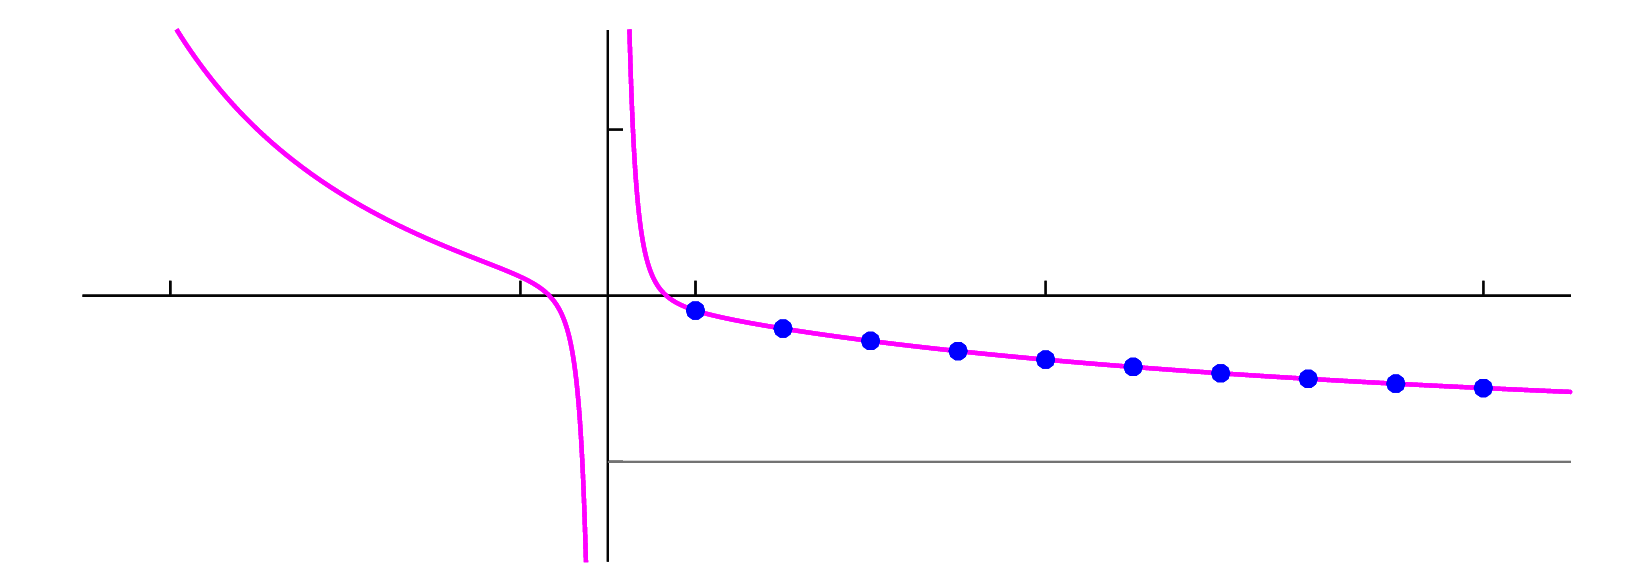
\includegraphics[width=14cm,height=5cm]{fig_exemplo_sequencia_por_funcao_racional}
\end{picture}%
\begin{picture}(396,141)(0,0)
\fontsize{10}{0}\selectfont\put(40.8522,62.6597){\makebox(0,0)[t]{\textcolor[rgb]{0.15,0.15,0.15}{{-5}}}}
\fontsize{10}{0}\selectfont\put(124.891,62.6597){\makebox(0,0)[t]{\textcolor[rgb]{0.15,0.15,0.15}{{-1}}}}
\fontsize{10}{0}\selectfont\put(166.911,62.6597){\makebox(0,0)[t]{\textcolor[rgb]{0.15,0.15,0.15}{{1}}}}
\fontsize{10}{0}\selectfont\put(250.95,62.6597){\makebox(0,0)[t]{\textcolor[rgb]{0.15,0.15,0.15}{{5}}}}
\fontsize{10}{0}\selectfont\put(355.998,62.6597){\makebox(0,0)[t]{\textcolor[rgb]{0.15,0.15,0.15}{{10}}}}
\fontsize{10}{0}\selectfont\put(140.899,30.2717){\makebox(0,0)[r]{\textcolor[rgb]{0.15,0.15,0.15}{{-5}}}}
\fontsize{10}{0}\selectfont\put(140.899,109.996){\makebox(0,0)[r]{\textcolor[rgb]{0.15,0.15,0.15}{{5}}}}
\fontsize{10}{0}\selectfont\put(156.406,121.955){\makebox(0,0)[l]{\textcolor[rgb]{0,0,0}{{$f(x)$}}}}
\fontsize{10}{0}\selectfont\put(313.979,42.2303){\makebox(0,0)[tl]{\textcolor[rgb]{0,0,0}{{$a_k$}}}}
\end{picture}
